%ch.tex


\chapter{The semantic web}
\begin{center}
{\small\em Where are we; how did we get here; and where are we going?}
\end{center}

\begin{figure}[tbp]
\begin{center}
{ 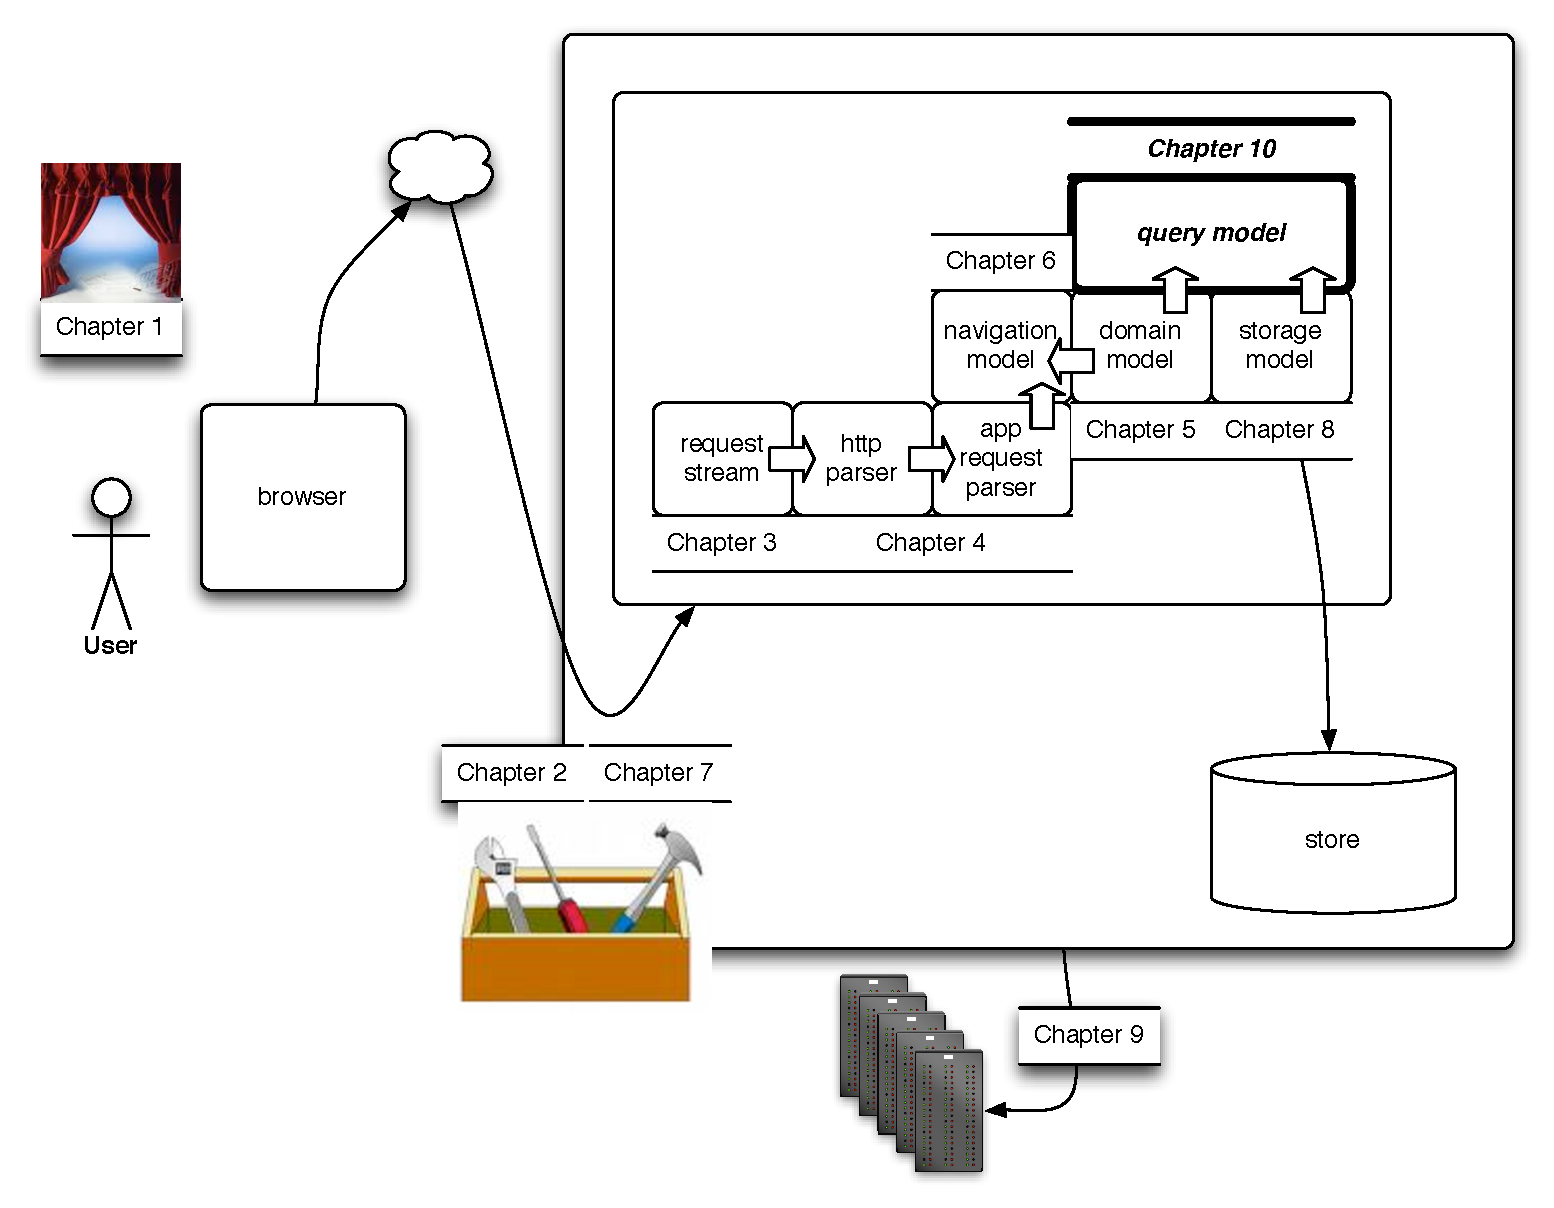
\includegraphics[scale=.35]{/Users/lgm/work/src/projex/biosimilarity/trace/src/main/book/content/figures/MonadicDesignPatternsChapterMapFocus10.pdf} }
\caption{ Chapter map }
\end{center}
\end{figure}

\section{Referential transparency}

In the interest of complete transparency, it is important for me to be
clear about my position on the current approach to the semantic
web. As early as 2004 i appeared in print as stating a complete lack
of confidence regarding meta-data, tags and ontology-based
approaches. Despite the attention and intense efforts around
technologies like \texttt{OWL}, i am unaware of major success
stories. The funny thing is, the same could be said of similar sorts
of efforts underway two decades before that, such as \texttt{KIF}, and
those two decades before that. i realize this is a controversial
position. However, since i worked one floor above Doug Lenat's team at
MCC, i feel i have a particular vantage point some 30 years on to ask,
so what has CyC done for you lately? In my humble opinion, the theory
of programming language semantics, especially compositional accounts
as found in $\lambda$-calculus and $\pi$-calculus, is currently the
best foundation we have for a theory we have of semantics, period.  As
such it constitutes the most sound basis for a good account of
\emph{knowledge representation}.

To make good on this claim, i want to illustrate how the monadic
techniques provide a new foundation for search on a semantic basis. In
particular, what we will see in the following sections of the
concluding chapter is how to use monads to search for programs in our
toy language on the basis of their structure and their
\emph{behavior}! Despite the fact that the open source movement has
created such a demand for higher-level techniques to search code
repositories, at present writing, i am unaware of any system, not
\texttt{Hoogle}, not \texttt{Merobase}, not \texttt{Google Codebase},
nor any of the other of several dozen efforts in this direction, that
offer this feature. Yet, the monadic design pattern not only makes it
clear that such a feature is a possibility, it makes the organization
of the code to do it perfectly tractable. i cannot imagine a more
powerful argument for the efficacy of this technique for structuring
functional programs.

\paragraph{A little motivation}

The next couple of sections will introduce some a little more
apparatus. Hopefully, by now, the reader is convinced of the value of
the more standard theoretical presentations of this kind of material
if for no other reason than the evident compression it affords. That
said, we recognize the need to ground the introduction of new
apparatus in good use cases. The discussion above can be turned
directly into a use case. The central point of this chapter is to
develop a query language for searching for programs in our toy
language. Following the analogy we established at the outset of this
book between \lstinline[language=SQL,mathescape=true]!select ... from ... where ...! and
\lstinline[language=Scala,mathescape=true]!for!-comprehensions, this
query language will allow users to write queries of the form

\begin{lstlisting}[language=Scala,mathescape=true]
  for( p <- d if c ) yield e
\end{lstlisting}

where \lstinline[language=Scala,mathescape=true]!p! is a pattern,
\lstinline[language=Scala,mathescape=true]!d! is an interface to a
data source and \lstinline[language=Scala,mathescape=true]!c! is a
predicate constraining the structure and behavior of the program. We
will show how to programmatically derive the language of patterns and
the language of constraints from our toy language.

The first new piece of machinery we need to introduce is how to
compose monads.


\section{Composing monads}

In all of the preceding chapters we deferred one of the most important
questions: do monads themselves compose? After all, if monad is the
proposal to replace the notion of object, and the primary criticism of
the notion of object is its lack of support for composition, hadn't we
better check that monads compose?

Intriguingly, monads do not automatically compose. That is, if
\lstinline[language=Scala,mathescape=true]!F $=$ (F, unit$_F$, mult$_F$)!
and \lstinline[language=Scala,mathescape=true]!G $=$ (G, unit$_G$, mult$_G$)!
are monads it does not necessarily follow that

\begin{lstlisting}[language=Scala,mathescape=true]
  F $\circ$ G $\stackrel{def}{=}$ (F $\circ$ G, unit$_F$ $\circ$ unit$_G$, mult$_f$ $\circ$ mult$_G$)
\end{lstlisting}

(which we'll write simply as
\lstinline[language=Scala,mathescape=true]!F G! going forward) is a
monad. In \texttt{Haskell} this is one of the purposes of monad
transformers, to sketch out a compositional model for monads. Here, we
follow a different route. The internal structure of a monad nearly
dictates the simplest conditions under which
\lstinline[language=Scala,mathescape=true]!F G! forms a
monad. Consider the requirement of having a
\lstinline[language=Scala,mathescape=true]!mult! for
\lstinline[language=Scala,mathescape=true]!F G!. We need a natural
transformation from \lstinline[language=Scala,mathescape=true]!mult: F G F G => F G!.

The components we have to build this mult are primarily
\lstinline[language=Scala,mathescape=true]!mult$_F$! and
\lstinline[language=Scala,mathescape=true]!mult$_G$!. These act to
take \lstinline[language=Scala,mathescape=true]!F F => G! and
\lstinline[language=Scala,mathescape=true]!G G => G!, yet we have
\lstinline[language=Scala,mathescape=true]!F G F G! as our initial
type. Notice that if we had a way of swapping the interior
\lstinline[language=Scala,mathescape=true]!G F! to make it
\lstinline[language=Scala,mathescape=true]!F G!, that is, we had a map
of the form \lstinline[language=Scala,mathescape=true]!d : G F => F G!
(\lstinline[language=Scala,mathescape=true]!d! for distributive
because it distributes \lstinline[language=Scala,mathescape=true]!F!
across \lstinline[language=Scala,mathescape=true]!G!), then we could
chain up like so

\begin{diagram}
  F G F G & \rTo^{F\;d\;G} & F F G G & \rTo^{mult_F \; mult_G} & F G \\
\end{diagram}

It is natural therefore, to require a map like
\lstinline[language=Scala,mathescape=true]!d! in order to compose
monads. We can investigate whether this proposal scales by looking at
how it fairs when we have three monads,
\lstinline[language=Scala,mathescape=true]!F!,
\lstinline[language=Scala,mathescape=true]!G! and
\lstinline[language=Scala,mathescape=true]!H!. We insist on being
supplied with distributive maps
\lstinline[language=Scala,mathescape=true]!d$_1$ : G F => F G!,
\lstinline[language=Scala,mathescape=true]!d$_2$ : H G => G H!  and,
for good measure, \lstinline[language=Scala,mathescape=true]!d$_3$ : H F => F H!. These will give canonical monads
\lstinline[language=Scala,mathescape=true]!(F G)H! and
\lstinline[language=Scala,mathescape=true]!F (G H)!, but we cannot
ensure their equality. That is, we cannot ensure the higher level of
associativity. To get this we need to impose an additional set of
requirements. These requirements come down to making the following
diagram commute.

\begin{diagram}
        &              & G H F & \rTo^{Gd_3}   & G F H &                 &       \\
        & \ruTo^{d_2F} &       &               &       & \rdTo^{d_{1}H}  &       \\
  H G F &              &       &               &       &                 & F G H \\
        & \rdTo_{Hd_1} &       &               &        & \ruTo_{Fd_{2}} &       \\
        &              & H F G & \rTo^{d_{3}G} & F H G &                 &       \\
\end{diagram}

They are the coherence conditions, the conditions of good interaction
amongst the distributive maps. In fact, this is sufficient to scale
out to arbitrary collections of monads. That is, if for any pair of
monads in the collection we have a distributive map, and for any three
we have the switching condition above, then composition is completely
coherent and well defined. To illustrate that this is not just some
abstract mathematical gadget lets put it to work. 

\subsubsection{Preliminary}
First we will consider a single distributive map. We will look at this
in terms of two extremely simple monads, a DSL for forming arithmetic
expressions involving only addition, i.e. a monoid, and a monad for
collection, in this case
\lstinline[language=Scala,mathescape=true]!Set!.

\begin{lstlisting}[language=Scala]
  case class MonoidExpr[Element]( val e : List[Element] )
  class MMExpr[A] extends Monad[A,MonoidExpr] {
    override def unit( e : A ) = MonoidExpr( List( e ) )
    override def mult( mme : MonoidExpr[MonoidExpr[A]] ) =
    mme match {
      case MonoidExpr( Nil ) =>
         MonoidExpr( Nil )
      case MonoidExpr( mes ) => 
         MonoidExpr(
            ( Nil /: mes)( 
               { ( acc, me ) => me match { 
                   case MonoidExpr( es ) => acc +++ es 
                 } 
               } 
             )
         )
    }
  }
\end{lstlisting}

Now, what we need to construct is a map
\lstinline[language=Scala,mathescape=true]!d! that takes elements
inhabiting the type
\lstinline[language=Scala,mathescape=true]!MMExpr[Set[A]]! to elements
inhabiting the type
\lstinline[language=Scala,mathescape=true]!Set[MMExpr[A]]!.

The primary technique is what's called point-wise lifting of
operations. Consider a simple example, such as the element

\lstinline[language=Scala,mathescape=true]!e = MMExpr( List( Set( a$_1$, a$_2$ ), Set( b$_1$, b$_2$, b$_3$ ) ) )!.

This element represents the composition of two sets. We can turn this
into a set of compositions, by considering pairs of
\lstinline[language=Scala,mathescape=true]!a!'s with
\lstinline[language=Scala,mathescape=true]!b!'s. That is,

\begin{lstlisting}[language=Scala,mathescape=true]
  e match {
    case MMExpr( s$_1$ :: s$_2$ :: Nil ) => 
       Set(
          for( a <- s$_1$; b <- s$_2$ )
          yield { MMExpr( List( a, b ) ) }
       )
    case ...
    }
\end{lstlisting}

This is exactly the type we want.

TBD
\section{How our web framework enables different kinds of application queries}

\subsubsection{An alternative presentation}

If you recall, there's an alternative way to present monads that are
algebras, like our monoid monad. Algebras are presented in terms of
generators and relations. In our case the generators presentation is
really just a grammar for monoid expressions.

\begin{mathpar}
  \inferrule* [lab=expression] {} {{m,n} ::=}
  \and
  \inferrule* [lab=identity element] {} {e}
  \and
  \inferrule* [lab=generators] {} {\;| \; g_1 \; | \; ... \; | \; g_n}
  \and
  \inferrule* [lab=monoid-multiplication] {} {\;| \; m * n}
\end{mathpar} 

This is subject to the following constraints, meaning that we will
treat syntactic expressions of certain forms as denoting the same
element of the monoid. To emphasize the nearly purely syntactic role
of these constraints we will use a different symbol for the
constraints. We also use the same symbol, $\equiv$, for the smallest equivalence
relation respecting these constraints.

\begin{mathpar}
  \inferrule* [lab=identity laws] {} {m * e \equiv m \equiv e * m}
  \and
  \inferrule* [lab=associativity] {} {m_1 * (m_2 * m_3) \equiv (m_1 * m_2) * m_3}
\end{mathpar} 

\paragraph{Logic: the set monad as an algebra}
In a similar manner, there is a language associated with the monad of
sets \emph{considered as an algebra}. This language is very familiar
to most programmers.

\begin{mathpar}
  \inferrule* [lab=expression] {} {{c,d} ::=}
  \and
  \inferrule* [lab=identity verity] {} {true}
  \and
  \inferrule* [lab=negation] {} {\;| \; \neg c}
  \and
  \inferrule* [lab=conjunction] {} {\;| \; c \& d}
\end{mathpar} 

Now, if we had a specific set in hand, say $L$ (which we'll call a
universe in the sequel), we can interpret the expressions in the this
language, aka formulae, in terms of operations on subsets of that
set. As with our compiler for the concrete syntax of the
$lambda$-calculus in chapter 1, we can express this translation very
compactly as

\begin{mathpar}
  \inferrule* {} {\meaningof{true} = L}
  \and
  \inferrule* {} {\meaningof{\neg c} = L \backslash c}
  \and 
  \inferrule* {} {\meaningof{c \& d} = \meaningof{c} \cap \meaningof{d}}
\end{mathpar}

Now, what's happening when we pull the monoid monad through the set
monad via a distributive map is this. First, the monoid monad
furnishes the universe, $L$, as the set of expressions generated by
the grammar. We'll denote this by $L(m)$. Then, we enrich the set of
formulae by the operations of the monoid \emph{acting on sets}.

\begin{mathpar}
  \inferrule* [lab=expression] {} {{c,d} ::=}
  \and
  \inferrule* [lab=identity verity] {} {true}
  \and
  \inferrule* [lab=negation] {} {\;| \; \neg c}
  \and
  \inferrule* [lab=conjunction] {} {\;| \; c \& d}
  \and
  \inferrule* [lab=identity verity] {} {\bf{e}}
  \and
  \inferrule* [lab=negation] {} {\;| \; \bf{g_1} \; | \; ... \; | \; \bf{g_n}}
  \and
  \inferrule* [lab=conjunction] {} {\;| \; c * d}
\end{mathpar} 

The identity element, $e$ and the generators of the monoid, $g_1$,
..., $g_n$, can be considered $0$-ary operations in the same way that
we usually consider constants as $0$-ary operations. To avoid
confusion between these elements and the \emph{logical formulae} that
pick them out of the crowd, we write the logical formulae in
$\bf{boldface}$.

Now, we can write our distributive map. Surprisingly, it is exactly a
meaning for our logic!

\begin{mathpar}
  \inferrule* {} {\meaningof{true} = L(m)}
  \and
  \inferrule* {} {\meaningof{\neg c} = L(m) \backslash c}
  \and 
  \inferrule* {} {\meaningof{c \& d} = \meaningof{c} \cap \meaningof{d}}
  \and
  \inferrule* {} {\meaningof{\bf{e}} = \{ m \; \in \; L(m) \; | \; m \equiv e \}}
  \and
  \inferrule* {} {\meaningof{\bf{g_i}} = \{ m \; \in \; L(m) \; | \; m \equiv g_i \}}
  \and
  \inferrule* {} {\meaningof{c*d} = \{ m \; \in \; L(m) \; | \; m \equiv m_1 * m_2, m_1 \; \in \; \meaningof{c}, m_2 \; \in \; \meaningof{d} \}}
\end{mathpar}

\paragraph{Primes: an application}
Before going any further, let's look at an example of how to use these
new operators. Suppose we wanted to pick out all the elements of the
monoid that were not expressible as a composition of other
elements. Obviously, for monoids with a finite set of generators, this
is exactly just the generators, so we could write $\bf{g_1} || ... ||
\bf{g_n}$\footnote{We get the disjunction, $||$, by the usual DeMorgan
  translation: $c || d \stackrel{def}{=} \neg( \neg c \& \neg
  d)$}. However, when the set of generators is not finite, as it is
when the monoid is the integers under multiplication, we need another
way to write this down. That's where our other operators come in
handy. A moment's thought suggests that we could say that since $true$
denotes any possible element in the monoid, an element is not a
composition using negation plus our composition formula, i.e. $\neg
(true * true)$. This is a little overkill, however. We just want to
eliminate non-trivial compositions. We know how to express the
identity element, that's $\bf{e}$, so we are interested in those
elements that are not the identity, i.e. $\neg \bf{e}$. Then a formula
that eliminates compositions of non-trivial elements is spelled out
$\neg (\neg e * \neg e)$. Finally, we want to eliminate the identity
as a solution. So, we arrive at $\neg (\neg e * \neg e) \& \neg
e$. There, that formula picks out the \emph{primes} of \emph{any}
monoid.

\paragraph{Summary}

What have we done? We've illustrated a specific distributive map, one
that pulls the set monad through the monoid monad. We've shown that
this particular distributive map coincides with giving a semantics to
a particular logic, one whose structure is derived solely from the
shape of the collection monad, i.e. set, and the shape of the term
language, in this case monoid.

\subsubsection{Iterating the design pattern}

The whole point of working in this manner is that by virtue of its
compositional structure it provides a much higher level of abstraction
and greater opportunities for reuse. To illustrate the point, we will
now iterate the construction using our toy language, the
$lambda$-calculus, as the term language. As we saw in chapter 1, the
$lambda$-calculus also has a generators and relations
presentation. Unlike a monoid, however, the lambda calculus has
another piece of machinery: reduction! In addition to structural
equivalence of terms (which is a bi-directional relation) there is the
$beta$-reduction rule that captures the \emph{behavioral} aspect of
the lambda calculus.

It is key to understand this underlying structure of language
definitions. In essence, when a DSL is purely about structure it is
presented entirely in terms of generators (read a grammar) and
relations (like the monoid laws). When the DSL is also about behavior,
i.e. the terms in the language somehow express some kind of
computation, then the language has a third component, some kind of
reduction relation. \footnote{In some sense this is one of the central
  contributions of the theory of computation back to
  mathematics. Algebraists have known for a long time about generators
  and relations presentations of algebraic structures (of which
  algebraic data types are a subset). This collective wisdom is
  studied, for example, in the field of universal
  algebra. Computational models like the $lambda$-calculus and more
  recently the process calculi, like Milner's $\pi$-calculus or
  Cardelli and Gordon's ambient calculus, take this presentation one
  step further and add a set of conditional rewrite rules to express
  the computational content of the model. It was Milner who first
  recognized this particular decomposition of language definitions in
  his seminal paper, Functions as Processes, where he reformulated the
  presentation $\pi$-calculus along these lines.} This organization,
this common factoring of the specification of a language, makes it
possible to factor code that handles a wide range of semantic
features. The logic we derive below provides a great example.

\section{Searching for programs}

TBD

% \section{Existence problems}
% We begin with some metamathematics.
% All problems about the existence of maps can be cast into one of the
% following two forms, which are in a sense mutually dual.

% \noindent
% {\bf The Extension Problem}\index{extension problem} \    %%% NB index entry tag
% Given an inclusion $ A \stackrel{i}{\hookrightarrow} X $, and a map
% $ A \stackrel{f}{\rightarrow} Y $,
% does there exist a map $f^{\dagger}:X\to Y$ such that
% $f^{\dagger}$ agrees with $f$ on $A$?

% Here the appropriate source category for maps should be clear from the
% context and, moreover, commutativity through a
% candidate $f^{\dagger}$ is precisely
% the restriction requirement; that is,
% $$f^{\dagger}   :  f^{\dagger}\circ i = f^{\dagger}|_A = f\,. $$
% If such an $f^{\dagger}$ exists\footnote{${}^{\dagger}$ suggests striving
% for perfection, crusading}, then it is called an {\bf
% extension}\index{extension!of a map|bi} of $f$ and is said to {\bf
% extend}\index{extend|bi} $f$. In any diagrams, the presence of
% a dotted arrow or an arrow carrying a ? indicates a pious hope, in no way
% begging the question of its existence. Note that we shall usually
% omit $\circ$ from composite maps.

% \noindent
% {\bf The Lifting Problem}\index{lifting problem} \
% Given a pair of maps $E \stackrel{p}{\rightarrow}B$ and $X \stackrel{f}
% {\rightarrow} B $,
% does there exist a map $f^{\circ} : X \to E$, with
% $pf^{\circ} = f  $?


% That {\em all\/} existence problems about maps are essentially of one
% type or
% the other from these two is seen as follows. Evidently, all existence problems
% are representable by triangular diagrams\index{triangular diagrams} and it
% is easily seen that there are only these six possibilities:
% \begin{center}\begin{picture}(300,70)  %augch2 75
% \put(5,60){\vector(1,0){30}}
% \put(55,60){\vector(1,0){30}}
% \put(135,60){\vector(-1,0){30}}
% \put(185,60){\vector(-1,0){30}}
% \put(235,60){\vector(-1,0){30}}
% \put(285,60){\vector(-1,0){30}}
% \put(0,55){\vector(0,-1){30}}
% \put(50,55){\vector(0,-1){30}}
% \put(100,25){\vector(0,1){30}}
% \put(150,25){\vector(0,1){30}}
% \put(200,55){\vector(0,-1){30}}
% \put(250,55){\vector(0,-1){30}}
% \put(28,33){\small ?}
% \put(78,33){\small ?}
% \put(128,33){\small ?}
% \put(178,33){\small ?}
% \put(228,33){\small ?}
% \put(278,33){\small ?}
% \put(10,3){\bf 1}
% \put(60,3){\bf 2}
% \put(110,3){\bf 3}
% \put(160,3){\bf 4}
% \put(210,3){\bf 5}
% \put(260,3){\bf 6}
% \put(35,55){\vector(-1,-1){30}}
% \put(155,25){\vector(1,1){30}}
% \put(135,55){\vector(-1,-1){30}}
% \put(55,25){\vector(1,1){30}}
% \put(235,55){\vector(-1,-1){30}}
% \put(255,25){\vector(1,1){30}}
% \end{picture}\end{center}



% \begin{figure}
% \begin{picture}(300,220)(0,0)
% \put(-20,-20){\resizebox{20 cm}{!}{\includegraphics{3dpdf}}}
% \put(260,-10){\resizebox{15 cm}{!}{\includegraphics{contpdf}}}
% \put(220,80){$\beta$}
% \put(400,-10){$N$}
% \put(260,170){$\beta$}
% \put(90,15){$N$}
% \end{picture}
% \caption{{\em The log-gamma family of densities with central mean
% $<N> \, = \frac{1}{2}$ as a surface and as a contour plot. }}
% \label{pdf}
% \end{figure}

\newpage
